\documentclass[twoside]{book}

% Packages required by doxygen
\usepackage{fixltx2e}
\usepackage{calc}
\usepackage{doxygen}
\usepackage[export]{adjustbox} % also loads graphicx
\usepackage{graphicx}
\usepackage[utf8]{inputenc}
\usepackage{makeidx}
\usepackage{multicol}
\usepackage{multirow}
\PassOptionsToPackage{warn}{textcomp}
\usepackage{textcomp}
\usepackage[nointegrals]{wasysym}
\usepackage[table]{xcolor}

% Font selection
\usepackage[T1]{fontenc}
\usepackage[scaled=.90]{helvet}
\usepackage{courier}
\usepackage{amssymb}
\usepackage{sectsty}
\renewcommand{\familydefault}{\sfdefault}
\allsectionsfont{%
  \fontseries{bc}\selectfont%
  \color{darkgray}%
}
\renewcommand{\DoxyLabelFont}{%
  \fontseries{bc}\selectfont%
  \color{darkgray}%
}
\newcommand{\+}{\discretionary{\mbox{\scriptsize$\hookleftarrow$}}{}{}}

% Page & text layout
\usepackage{geometry}
\geometry{%
  a4paper,%
  top=2.5cm,%
  bottom=2.5cm,%
  left=2.5cm,%
  right=2.5cm%
}
\tolerance=750
\hfuzz=15pt
\hbadness=750
\setlength{\emergencystretch}{15pt}
\setlength{\parindent}{0cm}
\setlength{\parskip}{3ex plus 2ex minus 2ex}
\makeatletter
\renewcommand{\paragraph}{%
  \@startsection{paragraph}{4}{0ex}{-1.0ex}{1.0ex}{%
    \normalfont\normalsize\bfseries\SS@parafont%
  }%
}
\renewcommand{\subparagraph}{%
  \@startsection{subparagraph}{5}{0ex}{-1.0ex}{1.0ex}{%
    \normalfont\normalsize\bfseries\SS@subparafont%
  }%
}
\makeatother

% Headers & footers
\usepackage{fancyhdr}
\pagestyle{fancyplain}
\fancyhead[LE]{\fancyplain{}{\bfseries\thepage}}
\fancyhead[CE]{\fancyplain{}{}}
\fancyhead[RE]{\fancyplain{}{\bfseries\leftmark}}
\fancyhead[LO]{\fancyplain{}{\bfseries\rightmark}}
\fancyhead[CO]{\fancyplain{}{}}
\fancyhead[RO]{\fancyplain{}{\bfseries\thepage}}
\fancyfoot[LE]{\fancyplain{}{}}
\fancyfoot[CE]{\fancyplain{}{}}
\fancyfoot[RE]{\fancyplain{}{\bfseries\scriptsize Generated by Doxygen }}
\fancyfoot[LO]{\fancyplain{}{\bfseries\scriptsize Generated by Doxygen }}
\fancyfoot[CO]{\fancyplain{}{}}
\fancyfoot[RO]{\fancyplain{}{}}
\renewcommand{\footrulewidth}{0.4pt}
\renewcommand{\chaptermark}[1]{%
  \markboth{#1}{}%
}
\renewcommand{\sectionmark}[1]{%
  \markright{\thesection\ #1}%
}

% Indices & bibliography
\usepackage{natbib}
\usepackage[titles]{tocloft}
\setcounter{tocdepth}{3}
\setcounter{secnumdepth}{5}
\makeindex

% Hyperlinks (required, but should be loaded last)
\usepackage{ifpdf}
\ifpdf
  \usepackage[pdftex,pagebackref=true]{hyperref}
\else
  \usepackage[ps2pdf,pagebackref=true]{hyperref}
\fi
\hypersetup{%
  colorlinks=true,%
  linkcolor=blue,%
  citecolor=blue,%
  unicode%
}

% Custom commands
\newcommand{\clearemptydoublepage}{%
  \newpage{\pagestyle{empty}\cleardoublepage}%
}

\usepackage{caption}
\captionsetup{labelsep=space,justification=centering,font={bf},singlelinecheck=off,skip=4pt,position=top}

%===== C O N T E N T S =====

\begin{document}

% Titlepage & ToC
\hypersetup{pageanchor=false,
             bookmarksnumbered=true,
             pdfencoding=unicode
            }
\pagenumbering{roman}
\begin{titlepage}
\vspace*{7cm}
\begin{center}%
{\Large D\+A\+RK E\+V\+IL \\[1ex]\large 6 }\\
\vspace*{1cm}
{\large Generated by Doxygen 1.8.11}\\
\end{center}
\end{titlepage}
\clearemptydoublepage
\tableofcontents
\clearemptydoublepage
\pagenumbering{arabic}
\hypersetup{pageanchor=true}

%--- Begin generated contents ---
\chapter{Data Structure Index}
\section{Data Structures}
Here are the data structures with brief descriptions\+:\begin{DoxyCompactList}
\item\contentsline{section}{\hyperlink{structpersonnage}{personnage} \\*Struct for personnage }{\pageref{structpersonnage}}{}
\end{DoxyCompactList}

\chapter{File Index}
\section{File List}
Here is a list of all files with brief descriptions\+:\begin{DoxyCompactList}
\item\contentsline{section}{\hyperlink{main1_8c}{main1.\+c} \\*Test Program }{\pageref{main1_8c}}{}
\item\contentsline{section}{\hyperlink{perso_8c}{perso.\+c} \\*Test Program }{\pageref{perso_8c}}{}
\item\contentsline{section}{\hyperlink{perso_8h}{perso.\+h} }{\pageref{perso_8h}}{}
\end{DoxyCompactList}

\chapter{Data Structure Documentation}
\hypertarget{structpersonnage}{}\section{personnage Struct Reference}
\label{structpersonnage}\index{personnage@{personnage}}


struct for personnage  




{\ttfamily \#include $<$perso.\+h$>$}

\subsection*{Data Fields}
\begin{DoxyCompactItemize}
\item 
int \hyperlink{structpersonnage_a5f78a81264a0d479a023826b20b86173}{nvie}
\item 
int \hyperlink{structpersonnage_a6c5c952d4dc96ed7f6be22480cb5a4d0}{nscore}
\item 
S\+D\+L\+\_\+\+Surface $\ast$ \hyperlink{structpersonnage_a7e7c398ea690ec57a5fce13c80386cd4}{mat} \mbox{[}3\mbox{]}\mbox{[}4\mbox{]}
\item 
S\+D\+L\+\_\+\+Rect \hyperlink{structpersonnage_a8216e2ba9fa8840fd13e47f40ccf356d}{Positionmat}
\item 
int \hyperlink{structpersonnage_ad3316ca5e21971af05da3b10b0d18fb3}{d}
\item 
int \hyperlink{structpersonnage_acfac32928075716cc10265cfc9f551fc}{num}
\item 
double \hyperlink{structpersonnage_a9833848acdb28a307902c8e1682213d9}{vitesse}
\item 
double \hyperlink{structpersonnage_aa3dc1bee3cdaa742eac0d46f56ac8908}{acceleration}
\item 
S\+D\+L\+\_\+\+Surface $\ast$ \hyperlink{structpersonnage_a3a476ed3aa74ef4eb7ea482739443401}{vie}
\item 
S\+D\+L\+\_\+\+Surface $\ast$ \hyperlink{structpersonnage_ad1416e47a9921f214b01e8435d2ea476}{score}
\item 
int \hyperlink{structpersonnage_ad781b14c9d0a4f927e6471b9cf1234df}{up}
\end{DoxyCompactItemize}


\subsection{Detailed Description}
struct for personnage 

Definition at line 12 of file perso.\+h.



\subsection{Field Documentation}
\index{personnage@{personnage}!acceleration@{acceleration}}
\index{acceleration@{acceleration}!personnage@{personnage}}
\subsubsection[{\texorpdfstring{acceleration}{acceleration}}]{\setlength{\rightskip}{0pt plus 5cm}double personnage\+::acceleration}\hypertarget{structpersonnage_aa3dc1bee3cdaa742eac0d46f56ac8908}{}\label{structpersonnage_aa3dc1bee3cdaa742eac0d46f56ac8908}


Definition at line 21 of file perso.\+h.

\index{personnage@{personnage}!d@{d}}
\index{d@{d}!personnage@{personnage}}
\subsubsection[{\texorpdfstring{d}{d}}]{\setlength{\rightskip}{0pt plus 5cm}int personnage\+::d}\hypertarget{structpersonnage_ad3316ca5e21971af05da3b10b0d18fb3}{}\label{structpersonnage_ad3316ca5e21971af05da3b10b0d18fb3}


Definition at line 18 of file perso.\+h.

\index{personnage@{personnage}!mat@{mat}}
\index{mat@{mat}!personnage@{personnage}}
\subsubsection[{\texorpdfstring{mat}{mat}}]{\setlength{\rightskip}{0pt plus 5cm}S\+D\+L\+\_\+\+Surface$\ast$ personnage\+::mat\mbox{[}3\mbox{]}\mbox{[}4\mbox{]}}\hypertarget{structpersonnage_a7e7c398ea690ec57a5fce13c80386cd4}{}\label{structpersonnage_a7e7c398ea690ec57a5fce13c80386cd4}
Surface 

Definition at line 16 of file perso.\+h.

\index{personnage@{personnage}!nscore@{nscore}}
\index{nscore@{nscore}!personnage@{personnage}}
\subsubsection[{\texorpdfstring{nscore}{nscore}}]{\setlength{\rightskip}{0pt plus 5cm}int personnage\+::nscore}\hypertarget{structpersonnage_a6c5c952d4dc96ed7f6be22480cb5a4d0}{}\label{structpersonnage_a6c5c952d4dc96ed7f6be22480cb5a4d0}


Definition at line 15 of file perso.\+h.

\index{personnage@{personnage}!num@{num}}
\index{num@{num}!personnage@{personnage}}
\subsubsection[{\texorpdfstring{num}{num}}]{\setlength{\rightskip}{0pt plus 5cm}int personnage\+::num}\hypertarget{structpersonnage_acfac32928075716cc10265cfc9f551fc}{}\label{structpersonnage_acfac32928075716cc10265cfc9f551fc}


Definition at line 19 of file perso.\+h.

\index{personnage@{personnage}!nvie@{nvie}}
\index{nvie@{nvie}!personnage@{personnage}}
\subsubsection[{\texorpdfstring{nvie}{nvie}}]{\setlength{\rightskip}{0pt plus 5cm}int personnage\+::nvie}\hypertarget{structpersonnage_a5f78a81264a0d479a023826b20b86173}{}\label{structpersonnage_a5f78a81264a0d479a023826b20b86173}


Definition at line 14 of file perso.\+h.

\index{personnage@{personnage}!Positionmat@{Positionmat}}
\index{Positionmat@{Positionmat}!personnage@{personnage}}
\subsubsection[{\texorpdfstring{Positionmat}{Positionmat}}]{\setlength{\rightskip}{0pt plus 5cm}S\+D\+L\+\_\+\+Rect personnage\+::\+Positionmat}\hypertarget{structpersonnage_a8216e2ba9fa8840fd13e47f40ccf356d}{}\label{structpersonnage_a8216e2ba9fa8840fd13e47f40ccf356d}
Rectangle 

Definition at line 17 of file perso.\+h.

\index{personnage@{personnage}!score@{score}}
\index{score@{score}!personnage@{personnage}}
\subsubsection[{\texorpdfstring{score}{score}}]{\setlength{\rightskip}{0pt plus 5cm}S\+D\+L\+\_\+\+Surface$\ast$ personnage\+::score}\hypertarget{structpersonnage_ad1416e47a9921f214b01e8435d2ea476}{}\label{structpersonnage_ad1416e47a9921f214b01e8435d2ea476}


Definition at line 23 of file perso.\+h.

\index{personnage@{personnage}!up@{up}}
\index{up@{up}!personnage@{personnage}}
\subsubsection[{\texorpdfstring{up}{up}}]{\setlength{\rightskip}{0pt plus 5cm}int personnage\+::up}\hypertarget{structpersonnage_ad781b14c9d0a4f927e6471b9cf1234df}{}\label{structpersonnage_ad781b14c9d0a4f927e6471b9cf1234df}


Definition at line 24 of file perso.\+h.

\index{personnage@{personnage}!vie@{vie}}
\index{vie@{vie}!personnage@{personnage}}
\subsubsection[{\texorpdfstring{vie}{vie}}]{\setlength{\rightskip}{0pt plus 5cm}S\+D\+L\+\_\+\+Surface$\ast$ personnage\+::vie}\hypertarget{structpersonnage_a3a476ed3aa74ef4eb7ea482739443401}{}\label{structpersonnage_a3a476ed3aa74ef4eb7ea482739443401}


Definition at line 22 of file perso.\+h.

\index{personnage@{personnage}!vitesse@{vitesse}}
\index{vitesse@{vitesse}!personnage@{personnage}}
\subsubsection[{\texorpdfstring{vitesse}{vitesse}}]{\setlength{\rightskip}{0pt plus 5cm}double personnage\+::vitesse}\hypertarget{structpersonnage_a9833848acdb28a307902c8e1682213d9}{}\label{structpersonnage_a9833848acdb28a307902c8e1682213d9}


Definition at line 20 of file perso.\+h.



The documentation for this struct was generated from the following file\+:\begin{DoxyCompactItemize}
\item 
\hyperlink{perso_8h}{perso.\+h}\end{DoxyCompactItemize}

\chapter{File Documentation}
\hypertarget{main1_8c}{}\section{main1.\+c File Reference}
\label{main1_8c}\index{main1.\+c@{main1.\+c}}


Test Program.  


{\ttfamily \#include $<$stdio.\+h$>$}\\*
{\ttfamily \#include $<$stdlib.\+h$>$}\\*
{\ttfamily \#include $<$S\+D\+L/\+S\+D\+L.\+h$>$}\\*
{\ttfamily \#include $<$S\+D\+L/\+S\+D\+L\+\_\+image.\+h$>$}\\*
{\ttfamily \#include $<$S\+D\+L/\+S\+D\+L\+\_\+ttf.\+h$>$}\\*
{\ttfamily \#include \char`\"{}perso.\+h\char`\"{}}\\*
Include dependency graph for main1.\+c\+:
\nopagebreak
\begin{figure}[H]
\begin{center}
\leavevmode
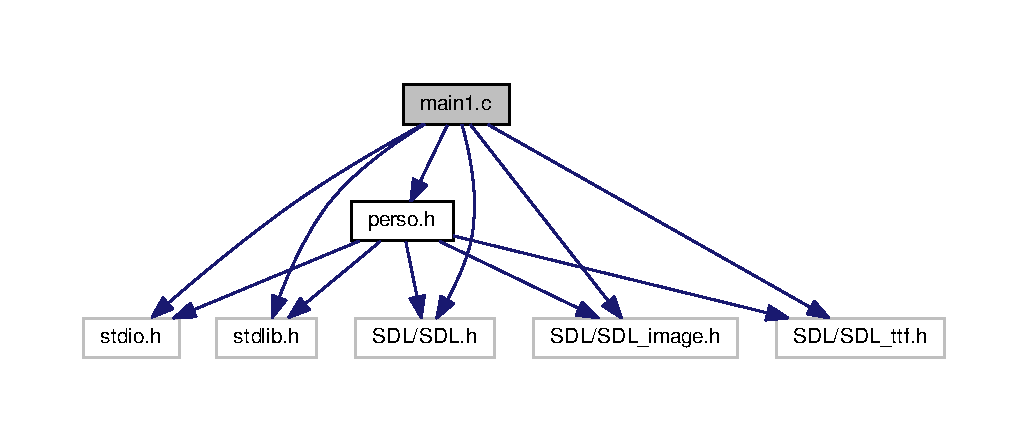
\includegraphics[width=350pt]{main1_8c__incl}
\end{center}
\end{figure}
\subsection*{Functions}
\begin{DoxyCompactItemize}
\item 
int \hyperlink{main1_8c_a0ddf1224851353fc92bfbff6f499fa97}{main} (int argc, char $\ast$argv\mbox{[}$\,$\mbox{]})
\end{DoxyCompactItemize}


\subsection{Detailed Description}
Test Program. 

\begin{DoxyAuthor}{Author}
dark evil Team 
\end{DoxyAuthor}
\begin{DoxyVersion}{Version}
6 
\end{DoxyVersion}
\begin{DoxyDate}{Date}
Apr 24, 2021
\end{DoxyDate}
Test program for \hyperlink{main1_8c}{main1.\+c} deplacement$\ast$ annimation $\ast$ saut $\ast$ 

\subsection{Function Documentation}
\index{main1.\+c@{main1.\+c}!main@{main}}
\index{main@{main}!main1.\+c@{main1.\+c}}
\subsubsection[{\texorpdfstring{main(int argc, char $\ast$argv[])}{main(int argc, char *argv[])}}]{\setlength{\rightskip}{0pt plus 5cm}int main (
\begin{DoxyParamCaption}
\item[{int}]{argc, }
\item[{char $\ast$}]{argv\mbox{[}$\,$\mbox{]}}
\end{DoxyParamCaption}
)}\hypertarget{main1_8c_a0ddf1224851353fc92bfbff6f499fa97}{}\label{main1_8c_a0ddf1224851353fc92bfbff6f499fa97}


Definition at line 26 of file main1.\+c.



References personnage\+::acceleration, afficherperso(), animate\+Entity(), blit\+Entity(), personnage\+::d, deplacer\+\_\+perso(), init\+\_\+perso(), personnage\+::mat, move\+Perso(), personnage\+::num, pers, saut(), personnage\+::score, personnage\+::up, and personnage\+::vie.


\begin{DoxyCode}
26                                        \{
27     SDL\_Surface *ecran=NULL; 
28      \textcolor{keywordtype}{int}  d; 
29     \hyperlink{structpersonnage}{personnage} \hyperlink{perso_8h_a9665deb0dbbab88867dd0328603d3f32}{pers}; 
30     Uint32 dt,t\_prev;
31 
32 
33 
34 SDL\_Init(SDL\_INIT\_VIDEO);
35 TTF\_Init(); 
36 \textcolor{keywordtype}{int} continuer=1;
37     SDL\_Event evenement; 
38     
39     ecran=SDL\_SetVideoMode(600,600,32,SDL\_HWSURFACE); 
40     
41 \textcolor{comment}{//creer et stocker des couleurs}
42 Uint32 red,green,blue, couleurCapeDuPersonnage;
43 couleurCapeDuPersonnage=SDL\_MapRGB(ecran->format,0,0,128);
44 red=SDL\_MapRGB(ecran->format,255,0,0);
45 
46 green=SDL\_MapRGB(ecran->format,0,255,0);
47 blue=SDL\_MapRGB(ecran->format,0,0,255);
48 SDL\_FillRect(ecran,NULL,couleurCapeDuPersonnage);
49 SDL\_Flip(ecran);
50 
51 
52 \textcolor{comment}{//le personnage}
53 \hyperlink{perso_8c_a21661aa89318d131d372cdacb5ef82c3}{init\_perso}(&pers);
54 
55     
56 
57 
58     
59 \textcolor{keywordflow}{while}(continuer)\{
60 
61 
62 SDL\_FillRect(ecran,NULL,couleurCapeDuPersonnage);
63 \hyperlink{perso_8c_a47ed0411b9adbc7543d3e80815cb3401}{afficherperso}(&pers,ecran);
64 
65 
66 
67 
68 \hyperlink{perso_8c_ae3c5c8505cfb2638fa312c5cb8e20aa5}{blitEntity}(&pers,ecran);
69     
70 SDL\_WaitEvent(&evenement);
71 t\_prev=SDL\_GetTicks();
72 
73 
74 \textcolor{keywordflow}{if}(evenement.type==SDL\_QUIT)
75 \{\textcolor{keywordflow}{break};\}    
76 
77 \textcolor{keywordflow}{if}(evenement.type==SDL\_KEYDOWN)\{
78         \textcolor{keywordflow}{if}(evenement.key.keysym.sym==SDLK\_LEFT)\{
79              d=1;
80                   pers.\hyperlink{structpersonnage_ad3316ca5e21971af05da3b10b0d18fb3}{d}=1;          
81 \} 
82       \textcolor{keywordflow}{else} 
83         \textcolor{keywordflow}{if} (evenement.key.keysym.sym==SDLK\_RIGHT)\{
84               d=0; 
85                
86                  pers.\hyperlink{structpersonnage_ad3316ca5e21971af05da3b10b0d18fb3}{d}=0;
87 \} 
88     \textcolor{keywordflow}{else} 
89         \textcolor{keywordflow}{if} (evenement.key.keysym.sym==SDLK\_a)\{
90 
91               d=2;
92               pers.\hyperlink{structpersonnage_ad3316ca5e21971af05da3b10b0d18fb3}{d}=2;       
93 \}
94  \textcolor{keywordflow}{else} 
95         \textcolor{keywordflow}{if} (evenement.key.keysym.sym==SDLK\_SPACE)
96 \{
97 
98 pers.\hyperlink{structpersonnage_aa3dc1bee3cdaa742eac0d46f56ac8908}{acceleration}+=0.005;
99 
100 \}
101 \textcolor{keywordflow}{else} \textcolor{keywordflow}{if} (evenement.key.keysym.sym==SDLK\_d)
102 \{    
103 
104 pers.\hyperlink{structpersonnage_aa3dc1bee3cdaa742eac0d46f56ac8908}{acceleration}-=0.01;
105 
106 \}
107 
108 \textcolor{keywordflow}{else} \textcolor{keywordflow}{if} (evenement.key.keysym.sym==SDLK\_UP)
109 \{
110 pers.\hyperlink{structpersonnage_a7e7c398ea690ec57a5fce13c80386cd4}{mat}[0][0]=pers.\hyperlink{structpersonnage_a7e7c398ea690ec57a5fce13c80386cd4}{mat}[0][1];
111 pers.\hyperlink{structpersonnage_ad781b14c9d0a4f927e6471b9cf1234df}{up}=1;
112 \hyperlink{perso_8c_aa512e7feb8c56d184403ca02f0c094a7}{saut}(&pers,dt,200);
113 
114  
115 \}
116 \textcolor{keywordflow}{if}(d>=0 && d<=1)
117      \{\hyperlink{perso_8c_ac29231e5ad237f14aa979bd358003dec}{deplacer\_perso}(d,&pers);\}
118 \hyperlink{perso_8c_aca4de1454b86bed715fb9f30706cd979}{movePerso}(&pers,dt);         
119 \hyperlink{perso_8c_ab3df315948613e2596ba989c3901ce00}{animateEntity}(&pers);
120 
121       
122 \}
123 dt=SDL\_GetTicks()-t\_prev;
124 
125 
126 
127 \}
128     
129 
130 SDL\_Surface *vie;
131         SDL\_Surface *score;
132 \textcolor{comment}{//Liberer la memoire}
133 
134 SDL\_FreeSurface(pers.\hyperlink{structpersonnage_a3a476ed3aa74ef4eb7ea482739443401}{vie});
135 SDL\_FreeSurface(pers.\hyperlink{structpersonnage_ad1416e47a9921f214b01e8435d2ea476}{score});
136 SDL\_FreeSurface(pers.\hyperlink{structpersonnage_a7e7c398ea690ec57a5fce13c80386cd4}{mat}[d][pers.\hyperlink{structpersonnage_acfac32928075716cc10265cfc9f551fc}{num}]);
137 SDL\_FreeSurface(ecran); 
138     TTF\_Quit();
139     SDL\_Quit();  
140     \textcolor{keywordflow}{return} 0; 
141     \}
\end{DoxyCode}


Here is the call graph for this function\+:
\nopagebreak
\begin{figure}[H]
\begin{center}
\leavevmode
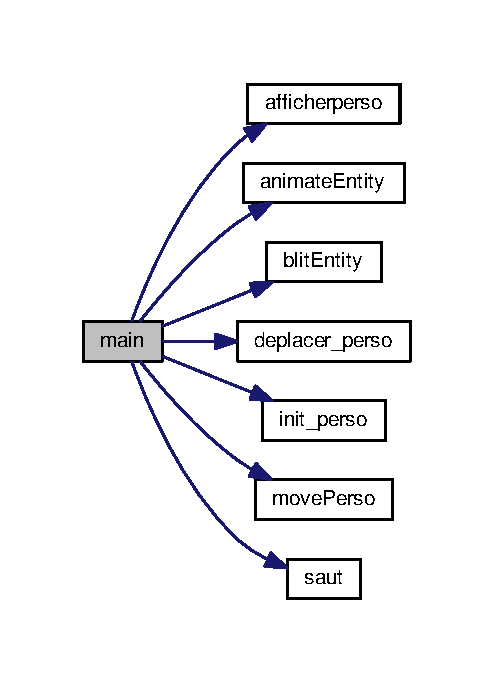
\includegraphics[width=237pt]{main1_8c_a0ddf1224851353fc92bfbff6f499fa97_cgraph}
\end{center}
\end{figure}



\hypertarget{perso_8c}{}\section{perso.\+c File Reference}
\label{perso_8c}\index{perso.\+c@{perso.\+c}}


Test Program.  


{\ttfamily \#include $<$stdio.\+h$>$}\\*
{\ttfamily \#include $<$stdlib.\+h$>$}\\*
{\ttfamily \#include $<$S\+D\+L/\+S\+D\+L.\+h$>$}\\*
{\ttfamily \#include $<$S\+D\+L/\+S\+D\+L\+\_\+image.\+h$>$}\\*
{\ttfamily \#include $<$S\+D\+L/\+S\+D\+L\+\_\+ttf.\+h$>$}\\*
{\ttfamily \#include \char`\"{}perso.\+h\char`\"{}}\\*
Include dependency graph for perso.\+c\+:
\nopagebreak
\begin{figure}[H]
\begin{center}
\leavevmode
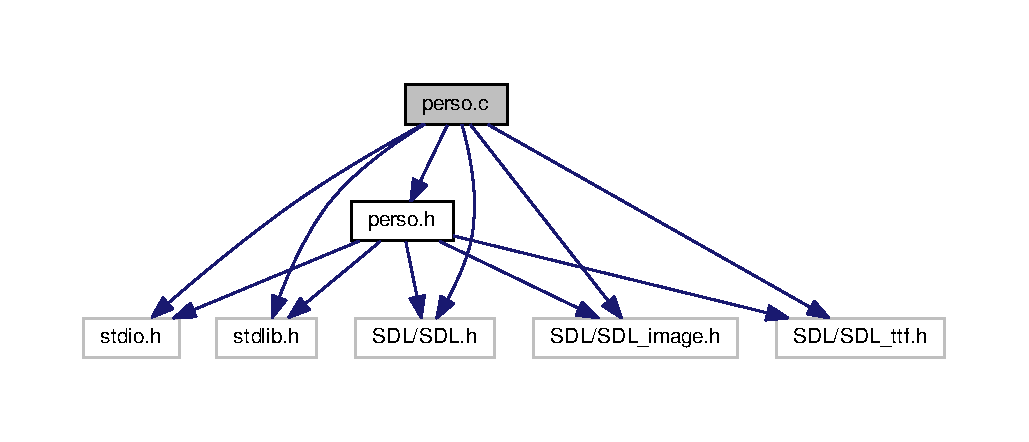
\includegraphics[width=350pt]{perso_8c__incl}
\end{center}
\end{figure}
\subsection*{Functions}
\begin{DoxyCompactItemize}
\item 
void \hyperlink{perso_8c_a21661aa89318d131d372cdacb5ef82c3}{init\+\_\+perso} (\hyperlink{structpersonnage}{personnage} $\ast$\hyperlink{perso_8h_a9665deb0dbbab88867dd0328603d3f32}{pers})
\begin{DoxyCompactList}\small\item\em To initialize the \hyperlink{perso_8c}{perso.\+c}. \end{DoxyCompactList}\item 
void \hyperlink{perso_8c_ab3df315948613e2596ba989c3901ce00}{animate\+Entity} (\hyperlink{structpersonnage}{personnage} $\ast$\hyperlink{perso_8h_a9665deb0dbbab88867dd0328603d3f32}{pers})
\begin{DoxyCompactList}\small\item\em to animate the personnage pers . \end{DoxyCompactList}\item 
void \hyperlink{perso_8c_ac29231e5ad237f14aa979bd358003dec}{deplacer\+\_\+perso} (int direction, \hyperlink{structpersonnage}{personnage} $\ast$\hyperlink{perso_8h_a9665deb0dbbab88867dd0328603d3f32}{pers})
\begin{DoxyCompactList}\small\item\em to move the personnage pers . \end{DoxyCompactList}\item 
void \hyperlink{perso_8c_aca4de1454b86bed715fb9f30706cd979}{move\+Perso} (\hyperlink{structpersonnage}{personnage} $\ast$\hyperlink{perso_8h_a9665deb0dbbab88867dd0328603d3f32}{pers}, Uint32 dt)
\begin{DoxyCompactList}\small\item\em to accelerate the personnage pers . \end{DoxyCompactList}\item 
void \hyperlink{perso_8c_ae3c5c8505cfb2638fa312c5cb8e20aa5}{blit\+Entity} (\hyperlink{structpersonnage}{personnage} $\ast$\hyperlink{perso_8h_a9665deb0dbbab88867dd0328603d3f32}{pers}, S\+D\+L\+\_\+\+Surface $\ast$ecran)
\begin{DoxyCompactList}\small\item\em to blit the surface of personnage pers . \end{DoxyCompactList}\item 
void \hyperlink{perso_8c_a47ed0411b9adbc7543d3e80815cb3401}{afficherperso} (\hyperlink{structpersonnage}{personnage} $\ast$\hyperlink{perso_8h_a9665deb0dbbab88867dd0328603d3f32}{pers}, S\+D\+L\+\_\+\+Surface $\ast$ecran)
\begin{DoxyCompactList}\small\item\em to show the personnage pers . \end{DoxyCompactList}\item 
void \hyperlink{perso_8c_aa512e7feb8c56d184403ca02f0c094a7}{saut} (\hyperlink{structpersonnage}{personnage} $\ast$\hyperlink{perso_8h_a9665deb0dbbab88867dd0328603d3f32}{pers}, int dt, int posint)
\begin{DoxyCompactList}\small\item\em jump the personnage pers . \end{DoxyCompactList}\end{DoxyCompactItemize}


\subsection{Detailed Description}
Test Program. 

\begin{DoxyAuthor}{Author}
dark evil Team 
\end{DoxyAuthor}
\begin{DoxyVersion}{Version}
6 
\end{DoxyVersion}
\begin{DoxyDate}{Date}
Apr 24, 2021
\end{DoxyDate}
Test program for perso saut $\ast$

\subsection{Function Documentation}
\index{perso.\+c@{perso.\+c}!afficherperso@{afficherperso}}
\index{afficherperso@{afficherperso}!perso.\+c@{perso.\+c}}
\subsubsection[{\texorpdfstring{afficherperso(personnage $\ast$pers, S\+D\+L\+\_\+\+Surface $\ast$ecran)}{afficherperso(personnage *pers, SDL_Surface *ecran)}}]{\setlength{\rightskip}{0pt plus 5cm}void afficherperso (
\begin{DoxyParamCaption}
\item[{{\bf personnage} $\ast$}]{pers, }
\item[{S\+D\+L\+\_\+\+Surface $\ast$}]{ecran}
\end{DoxyParamCaption}
)}\hypertarget{perso_8c_a47ed0411b9adbc7543d3e80815cb3401}{}\label{perso_8c_a47ed0411b9adbc7543d3e80815cb3401}


to show the personnage pers . 


\begin{DoxyParams}{Parameters}
{\em pers} & the personnage \\
\hline
\end{DoxyParams}
\begin{DoxyReturn}{Returns}
Nothing 
\end{DoxyReturn}


Definition at line 174 of file perso.\+c.



References personnage\+::score, and personnage\+::vie.


\begin{DoxyCode}
175 \{
176 pers->\hyperlink{structpersonnage_a3a476ed3aa74ef4eb7ea482739443401}{vie}=IMG\_Load(\textcolor{stringliteral}{"v1.png"});
177 SDL\_Rect vieposition;
178 vieposition.x=0;
179 vieposition.y=0;
180 SDL\_BlitSurface(pers->\hyperlink{structpersonnage_a3a476ed3aa74ef4eb7ea482739443401}{vie},NULL,ecran,&vieposition);
181 SDL\_Flip(ecran);
182 
183 TTF\_Font *fontTest;
184 fontTest=TTF\_OpenFont(\textcolor{stringliteral}{"arial.ttf"},22);
185 SDL\_Color fontColor=\{0,0,255\};
186 
187 \textcolor{comment}{//police1}
188 pers->\hyperlink{structpersonnage_ad1416e47a9921f214b01e8435d2ea476}{score}=TTF\_RenderText\_Solid(fontTest,\textcolor{stringliteral}{"Score :"},fontColor);
189 SDL\_Rect texte1Pos;
190 texte1Pos.x=0;
191 texte1Pos.y=70;
192 SDL\_BlitSurface(pers->\hyperlink{structpersonnage_ad1416e47a9921f214b01e8435d2ea476}{score},NULL,ecran,&texte1Pos);
193 SDL\_Flip(ecran);
194 
195 
196 
197 \}
\end{DoxyCode}


Here is the caller graph for this function\+:
\nopagebreak
\begin{figure}[H]
\begin{center}
\leavevmode
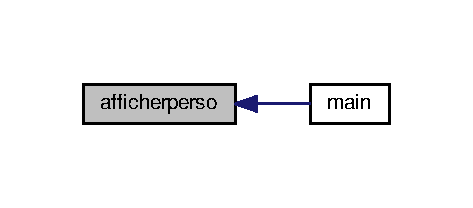
\includegraphics[width=227pt]{perso_8c_a47ed0411b9adbc7543d3e80815cb3401_icgraph}
\end{center}
\end{figure}


\index{perso.\+c@{perso.\+c}!animate\+Entity@{animate\+Entity}}
\index{animate\+Entity@{animate\+Entity}!perso.\+c@{perso.\+c}}
\subsubsection[{\texorpdfstring{animate\+Entity(personnage $\ast$pers)}{animateEntity(personnage *pers)}}]{\setlength{\rightskip}{0pt plus 5cm}void animate\+Entity (
\begin{DoxyParamCaption}
\item[{{\bf personnage} $\ast$}]{pers}
\end{DoxyParamCaption}
)}\hypertarget{perso_8c_ab3df315948613e2596ba989c3901ce00}{}\label{perso_8c_ab3df315948613e2596ba989c3901ce00}


to animate the personnage pers . 


\begin{DoxyParams}{Parameters}
{\em matrice} & \\
\hline
{\em pers} & the personnage \\
\hline
\end{DoxyParams}
\begin{DoxyReturn}{Returns}
Nothing 
\end{DoxyReturn}


Definition at line 93 of file perso.\+c.



References personnage\+::num.


\begin{DoxyCode}
94 \{
95 
96 \textcolor{keywordflow}{if}(pers->\hyperlink{structpersonnage_acfac32928075716cc10265cfc9f551fc}{num}==3)
97 pers->\hyperlink{structpersonnage_acfac32928075716cc10265cfc9f551fc}{num}=0;
98 \textcolor{keywordflow}{else} pers->\hyperlink{structpersonnage_acfac32928075716cc10265cfc9f551fc}{num}++;
99 
100 \}
\end{DoxyCode}


Here is the caller graph for this function\+:
\nopagebreak
\begin{figure}[H]
\begin{center}
\leavevmode
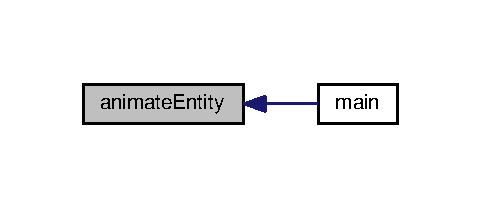
\includegraphics[width=231pt]{perso_8c_ab3df315948613e2596ba989c3901ce00_icgraph}
\end{center}
\end{figure}


\index{perso.\+c@{perso.\+c}!blit\+Entity@{blit\+Entity}}
\index{blit\+Entity@{blit\+Entity}!perso.\+c@{perso.\+c}}
\subsubsection[{\texorpdfstring{blit\+Entity(personnage $\ast$pers, S\+D\+L\+\_\+\+Surface $\ast$ecran)}{blitEntity(personnage *pers, SDL_Surface *ecran)}}]{\setlength{\rightskip}{0pt plus 5cm}void blit\+Entity (
\begin{DoxyParamCaption}
\item[{{\bf personnage} $\ast$}]{pers, }
\item[{S\+D\+L\+\_\+\+Surface $\ast$}]{ecran}
\end{DoxyParamCaption}
)}\hypertarget{perso_8c_ae3c5c8505cfb2638fa312c5cb8e20aa5}{}\label{perso_8c_ae3c5c8505cfb2638fa312c5cb8e20aa5}


to blit the surface of personnage pers . 


\begin{DoxyParams}{Parameters}
{\em pers} & the personnage \\
\hline
\end{DoxyParams}
\begin{DoxyReturn}{Returns}
Nothing 
\end{DoxyReturn}


Definition at line 157 of file perso.\+c.



References personnage\+::d, personnage\+::mat, personnage\+::num, and personnage\+::\+Positionmat.


\begin{DoxyCode}
158 \{
159 
160 SDL\_BlitSurface(pers->\hyperlink{structpersonnage_a7e7c398ea690ec57a5fce13c80386cd4}{mat}[pers->\hyperlink{structpersonnage_ad3316ca5e21971af05da3b10b0d18fb3}{d}][pers->\hyperlink{structpersonnage_acfac32928075716cc10265cfc9f551fc}{num}],NULL,ecran,&pers->
      \hyperlink{structpersonnage_a8216e2ba9fa8840fd13e47f40ccf356d}{Positionmat});
161 SDL\_Flip(ecran);
162 
163 \}
\end{DoxyCode}


Here is the caller graph for this function\+:
\nopagebreak
\begin{figure}[H]
\begin{center}
\leavevmode
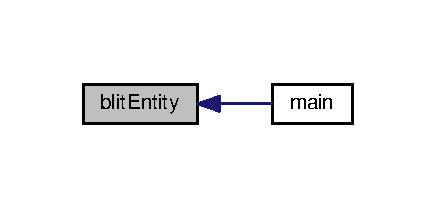
\includegraphics[width=209pt]{perso_8c_ae3c5c8505cfb2638fa312c5cb8e20aa5_icgraph}
\end{center}
\end{figure}


\index{perso.\+c@{perso.\+c}!deplacer\+\_\+perso@{deplacer\+\_\+perso}}
\index{deplacer\+\_\+perso@{deplacer\+\_\+perso}!perso.\+c@{perso.\+c}}
\subsubsection[{\texorpdfstring{deplacer\+\_\+perso(int direction, personnage $\ast$pers)}{deplacer_perso(int direction, personnage *pers)}}]{\setlength{\rightskip}{0pt plus 5cm}void deplacer\+\_\+perso (
\begin{DoxyParamCaption}
\item[{int}]{direction, }
\item[{{\bf personnage} $\ast$}]{pers}
\end{DoxyParamCaption}
)}\hypertarget{perso_8c_ac29231e5ad237f14aa979bd358003dec}{}\label{perso_8c_ac29231e5ad237f14aa979bd358003dec}


to move the personnage pers . 


\begin{DoxyParams}{Parameters}
{\em pers} & the personnage \\
\hline
\end{DoxyParams}
\begin{DoxyReturn}{Returns}
Nothing 
\end{DoxyReturn}


Definition at line 112 of file perso.\+c.



References personnage\+::\+Positionmat.


\begin{DoxyCode}
112                                                    \{
113     
114     \textcolor{keywordflow}{if}(direction==0)\{
115               
116               pers->\hyperlink{structpersonnage_a8216e2ba9fa8840fd13e47f40ccf356d}{Positionmat}.x+=25; 
117                    
118 \} 
119      \textcolor{keywordflow}{else} 
120          \textcolor{keywordflow}{if}(direction==1)\{ 
121                
122               pers->\hyperlink{structpersonnage_a8216e2ba9fa8840fd13e47f40ccf356d}{Positionmat}.x-=25; \}
123               
124 \textcolor{keywordflow}{else} \textcolor{keywordflow}{if}(direction==2)
125 \{
126 
127 pers->\hyperlink{structpersonnage_a8216e2ba9fa8840fd13e47f40ccf356d}{Positionmat}.x+=2;
128 
129 \}
130     
131 
132 
133 
134 \}
\end{DoxyCode}


Here is the caller graph for this function\+:
\nopagebreak
\begin{figure}[H]
\begin{center}
\leavevmode
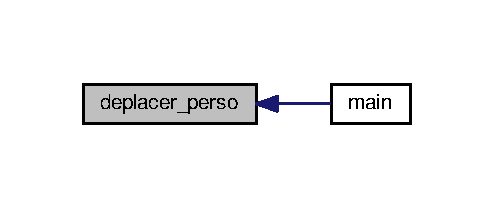
\includegraphics[width=237pt]{perso_8c_ac29231e5ad237f14aa979bd358003dec_icgraph}
\end{center}
\end{figure}


\index{perso.\+c@{perso.\+c}!init\+\_\+perso@{init\+\_\+perso}}
\index{init\+\_\+perso@{init\+\_\+perso}!perso.\+c@{perso.\+c}}
\subsubsection[{\texorpdfstring{init\+\_\+perso(personnage $\ast$pers)}{init_perso(personnage *pers)}}]{\setlength{\rightskip}{0pt plus 5cm}void init\+\_\+perso (
\begin{DoxyParamCaption}
\item[{{\bf personnage} $\ast$}]{pers}
\end{DoxyParamCaption}
)}\hypertarget{perso_8c_a21661aa89318d131d372cdacb5ef82c3}{}\label{perso_8c_a21661aa89318d131d372cdacb5ef82c3}


To initialize the \hyperlink{perso_8c}{perso.\+c}. 


\begin{DoxyParams}{Parameters}
{\em pers} & the personnage \\
\hline
{\em url} & the url of the image \\
\hline
\end{DoxyParams}
\begin{DoxyReturn}{Returns}
Nothing 
\end{DoxyReturn}


Definition at line 39 of file perso.\+c.



References personnage\+::acceleration, personnage\+::d, personnage\+::mat, personnage\+::nscore, personnage\+::num, personnage\+::nvie, personnage\+::\+Positionmat, personnage\+::up, and personnage\+::vitesse.


\begin{DoxyCode}
39                                  \{
40     pers->\hyperlink{structpersonnage_a7e7c398ea690ec57a5fce13c80386cd4}{mat}[0][0]=IMG\_Load(\textcolor{stringliteral}{"p.png"}); 
41         pers->\hyperlink{structpersonnage_a7e7c398ea690ec57a5fce13c80386cd4}{mat}[0][1]=IMG\_Load(\textcolor{stringliteral}{"p1.png"});
42         pers->\hyperlink{structpersonnage_a7e7c398ea690ec57a5fce13c80386cd4}{mat}[0][2]=IMG\_Load(\textcolor{stringliteral}{"p2.png"});
43         pers->\hyperlink{structpersonnage_a7e7c398ea690ec57a5fce13c80386cd4}{mat}[0][3]=IMG\_Load(\textcolor{stringliteral}{"p3.png"});  
44         pers->\hyperlink{structpersonnage_a7e7c398ea690ec57a5fce13c80386cd4}{mat}[1][0]=IMG\_Load(\textcolor{stringliteral}{"p4.png"});
45         pers->\hyperlink{structpersonnage_a7e7c398ea690ec57a5fce13c80386cd4}{mat}[1][1]=IMG\_Load(\textcolor{stringliteral}{"p5.png"});
46         pers->\hyperlink{structpersonnage_a7e7c398ea690ec57a5fce13c80386cd4}{mat}[1][2]=IMG\_Load(\textcolor{stringliteral}{"p6.png"});
47         pers->\hyperlink{structpersonnage_a7e7c398ea690ec57a5fce13c80386cd4}{mat}[1][3]=IMG\_Load(\textcolor{stringliteral}{"p7.png"});
48         pers->\hyperlink{structpersonnage_a7e7c398ea690ec57a5fce13c80386cd4}{mat}[2][0]=IMG\_Load(\textcolor{stringliteral}{"p10.png"});  
49         pers->\hyperlink{structpersonnage_a7e7c398ea690ec57a5fce13c80386cd4}{mat}[2][1]=IMG\_Load(\textcolor{stringliteral}{"p10.png"});
50         pers->\hyperlink{structpersonnage_a7e7c398ea690ec57a5fce13c80386cd4}{mat}[2][2]=IMG\_Load(\textcolor{stringliteral}{"p10.png"});
51         pers->\hyperlink{structpersonnage_a7e7c398ea690ec57a5fce13c80386cd4}{mat}[2][3]=IMG\_Load(\textcolor{stringliteral}{"p10.png"});
52 
53 pers->\hyperlink{structpersonnage_ad3316ca5e21971af05da3b10b0d18fb3}{d}=0;
54 pers->\hyperlink{structpersonnage_acfac32928075716cc10265cfc9f551fc}{num}=0;
55 pers->\hyperlink{structpersonnage_a8216e2ba9fa8840fd13e47f40ccf356d}{Positionmat}.x=0;
56 pers->\hyperlink{structpersonnage_a8216e2ba9fa8840fd13e47f40ccf356d}{Positionmat}.y=250;
57 pers->\hyperlink{structpersonnage_a5f78a81264a0d479a023826b20b86173}{nvie}=3; 
58 pers->\hyperlink{structpersonnage_a6c5c952d4dc96ed7f6be22480cb5a4d0}{nscore}=0; 
59 
60 pers->\hyperlink{structpersonnage_a9833848acdb28a307902c8e1682213d9}{vitesse}=5;
61 pers->\hyperlink{structpersonnage_aa3dc1bee3cdaa742eac0d46f56ac8908}{acceleration}=0;
62 pers->\hyperlink{structpersonnage_ad781b14c9d0a4f927e6471b9cf1234df}{up}=0;
63 
64 
65     
66 
67 
68 
69 
70 
71 
72 
73 
74 
75 \}
\end{DoxyCode}


Here is the caller graph for this function\+:
\nopagebreak
\begin{figure}[H]
\begin{center}
\leavevmode
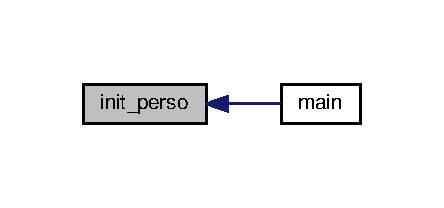
\includegraphics[width=213pt]{perso_8c_a21661aa89318d131d372cdacb5ef82c3_icgraph}
\end{center}
\end{figure}


\index{perso.\+c@{perso.\+c}!move\+Perso@{move\+Perso}}
\index{move\+Perso@{move\+Perso}!perso.\+c@{perso.\+c}}
\subsubsection[{\texorpdfstring{move\+Perso(personnage $\ast$pers, Uint32 dt)}{movePerso(personnage *pers, Uint32 dt)}}]{\setlength{\rightskip}{0pt plus 5cm}void move\+Perso (
\begin{DoxyParamCaption}
\item[{{\bf personnage} $\ast$}]{pers, }
\item[{Uint32}]{dt}
\end{DoxyParamCaption}
)}\hypertarget{perso_8c_aca4de1454b86bed715fb9f30706cd979}{}\label{perso_8c_aca4de1454b86bed715fb9f30706cd979}


to accelerate the personnage pers . 


\begin{DoxyParams}{Parameters}
{\em pers} & the personnage \\
\hline
\end{DoxyParams}
\begin{DoxyReturn}{Returns}
Nothing 
\end{DoxyReturn}


Definition at line 143 of file perso.\+c.



References personnage\+::acceleration, and personnage\+::vitesse.


\begin{DoxyCode}
144 \{
145 \textcolor{keywordtype}{double} dx;
146 dx=pers->\hyperlink{structpersonnage_a9833848acdb28a307902c8e1682213d9}{vitesse}*dt+0.5*pers->\hyperlink{structpersonnage_aa3dc1bee3cdaa742eac0d46f56ac8908}{acceleration}*dt*dt;
147 
148 \}
\end{DoxyCode}


Here is the caller graph for this function\+:
\nopagebreak
\begin{figure}[H]
\begin{center}
\leavevmode
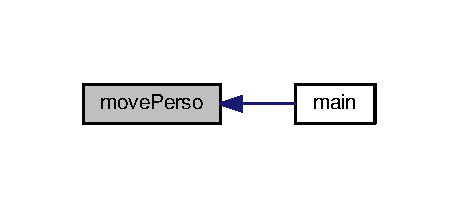
\includegraphics[width=220pt]{perso_8c_aca4de1454b86bed715fb9f30706cd979_icgraph}
\end{center}
\end{figure}


\index{perso.\+c@{perso.\+c}!saut@{saut}}
\index{saut@{saut}!perso.\+c@{perso.\+c}}
\subsubsection[{\texorpdfstring{saut(personnage $\ast$pers, int dt, int posint)}{saut(personnage *pers, int dt, int posint)}}]{\setlength{\rightskip}{0pt plus 5cm}void saut (
\begin{DoxyParamCaption}
\item[{{\bf personnage} $\ast$}]{pers, }
\item[{int}]{dt, }
\item[{int}]{posint}
\end{DoxyParamCaption}
)}\hypertarget{perso_8c_aa512e7feb8c56d184403ca02f0c094a7}{}\label{perso_8c_aa512e7feb8c56d184403ca02f0c094a7}


jump the personnage pers . 


\begin{DoxyParams}{Parameters}
{\em pers} & the personnage \\
\hline
\end{DoxyParams}
\begin{DoxyReturn}{Returns}
Nothing 
\end{DoxyReturn}


Definition at line 206 of file perso.\+c.



References personnage\+::acceleration, personnage\+::\+Positionmat, personnage\+::up, and personnage\+::vitesse.


\begin{DoxyCode}
207 \{
208 
209 \textcolor{keywordflow}{if}(pers->\hyperlink{structpersonnage_ad781b14c9d0a4f927e6471b9cf1234df}{up}==1)
210 \{
211 pers->\hyperlink{structpersonnage_a8216e2ba9fa8840fd13e47f40ccf356d}{Positionmat}.y-=80;
212 
213 
214 
215 \}
216 posint=pers->\hyperlink{structpersonnage_a8216e2ba9fa8840fd13e47f40ccf356d}{Positionmat}.y-=80;
217 
218 
219 \textcolor{keywordtype}{double} dx;
220 \textcolor{keywordflow}{if}(pers->\hyperlink{structpersonnage_a8216e2ba9fa8840fd13e47f40ccf356d}{Positionmat}.y==posint)
221 \{
222 
223 
224 pers->\hyperlink{structpersonnage_a8216e2ba9fa8840fd13e47f40ccf356d}{Positionmat}.y+=80;
225 
226 dx=0.5*pers->\hyperlink{structpersonnage_aa3dc1bee3cdaa742eac0d46f56ac8908}{acceleration} + 5*dt;
227 pers->\hyperlink{structpersonnage_a9833848acdb28a307902c8e1682213d9}{vitesse}-=dx;
228 \}
229 
230 
231 
232 
233 \}
\end{DoxyCode}


Here is the caller graph for this function\+:
\nopagebreak
\begin{figure}[H]
\begin{center}
\leavevmode
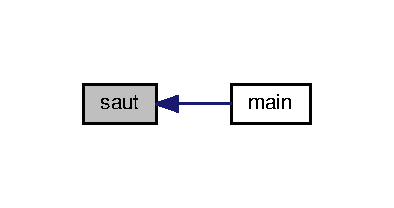
\includegraphics[width=189pt]{perso_8c_aa512e7feb8c56d184403ca02f0c094a7_icgraph}
\end{center}
\end{figure}



\hypertarget{perso_8h}{}\section{perso.\+h File Reference}
\label{perso_8h}\index{perso.\+h@{perso.\+h}}
{\ttfamily \#include $<$stdio.\+h$>$}\\*
{\ttfamily \#include $<$stdlib.\+h$>$}\\*
{\ttfamily \#include $<$S\+D\+L/\+S\+D\+L.\+h$>$}\\*
{\ttfamily \#include $<$S\+D\+L/\+S\+D\+L\+\_\+image.\+h$>$}\\*
{\ttfamily \#include $<$S\+D\+L/\+S\+D\+L\+\_\+ttf.\+h$>$}\\*
Include dependency graph for perso.\+h\+:
\nopagebreak
\begin{figure}[H]
\begin{center}
\leavevmode
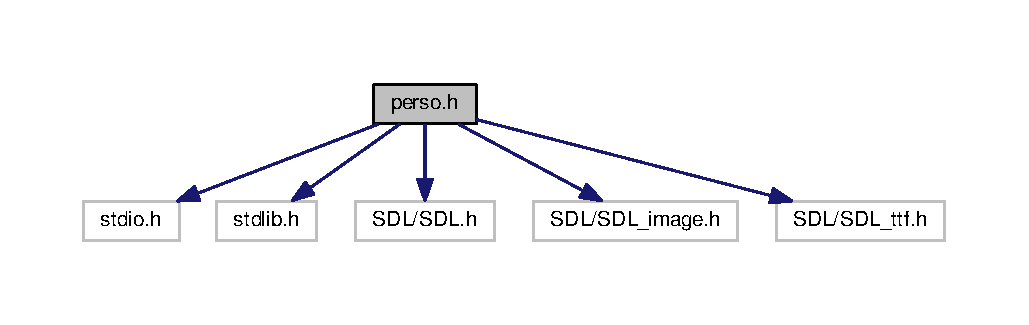
\includegraphics[width=350pt]{perso_8h__incl}
\end{center}
\end{figure}
This graph shows which files directly or indirectly include this file\+:
\nopagebreak
\begin{figure}[H]
\begin{center}
\leavevmode
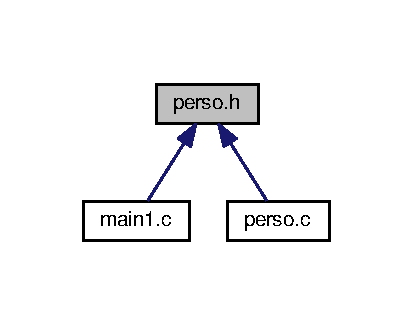
\includegraphics[width=198pt]{perso_8h__dep__incl}
\end{center}
\end{figure}
\subsection*{Data Structures}
\begin{DoxyCompactItemize}
\item 
struct \hyperlink{structpersonnage}{personnage}
\begin{DoxyCompactList}\small\item\em struct for personnage \end{DoxyCompactList}\end{DoxyCompactItemize}
\subsection*{Functions}
\begin{DoxyCompactItemize}
\item 
void \hyperlink{perso_8h_a21661aa89318d131d372cdacb5ef82c3}{init\+\_\+perso} (\hyperlink{structpersonnage}{personnage} $\ast$\hyperlink{perso_8h_a9665deb0dbbab88867dd0328603d3f32}{pers})
\begin{DoxyCompactList}\small\item\em To initialize the \hyperlink{perso_8c}{perso.\+c}. \end{DoxyCompactList}\item 
void \hyperlink{perso_8h_ac94dc8852307f2c897b9a1e6b3092314}{afficher\+\_\+perso} (\hyperlink{structpersonnage}{personnage} $\ast$\hyperlink{perso_8h_a9665deb0dbbab88867dd0328603d3f32}{pers})
\item 
void \hyperlink{perso_8h_ac29231e5ad237f14aa979bd358003dec}{deplacer\+\_\+perso} (int direction, \hyperlink{structpersonnage}{personnage} $\ast$\hyperlink{perso_8h_a9665deb0dbbab88867dd0328603d3f32}{pers})
\begin{DoxyCompactList}\small\item\em to move the personnage pers . \end{DoxyCompactList}\item 
void \hyperlink{perso_8h_aca4de1454b86bed715fb9f30706cd979}{move\+Perso} (\hyperlink{structpersonnage}{personnage} $\ast$\hyperlink{perso_8h_a9665deb0dbbab88867dd0328603d3f32}{pers}, Uint32 dt)
\begin{DoxyCompactList}\small\item\em to accelerate the personnage pers . \end{DoxyCompactList}\item 
void \hyperlink{perso_8h_ab3df315948613e2596ba989c3901ce00}{animate\+Entity} (\hyperlink{structpersonnage}{personnage} $\ast$\hyperlink{perso_8h_a9665deb0dbbab88867dd0328603d3f32}{pers})
\begin{DoxyCompactList}\small\item\em to animate the personnage pers . \end{DoxyCompactList}\item 
void \hyperlink{perso_8h_ae3c5c8505cfb2638fa312c5cb8e20aa5}{blit\+Entity} (\hyperlink{structpersonnage}{personnage} $\ast$\hyperlink{perso_8h_a9665deb0dbbab88867dd0328603d3f32}{pers}, S\+D\+L\+\_\+\+Surface $\ast$ecran)
\begin{DoxyCompactList}\small\item\em to blit the surface of personnage pers . \end{DoxyCompactList}\item 
void \hyperlink{perso_8h_a47ed0411b9adbc7543d3e80815cb3401}{afficherperso} (\hyperlink{structpersonnage}{personnage} $\ast$\hyperlink{perso_8h_a9665deb0dbbab88867dd0328603d3f32}{pers}, S\+D\+L\+\_\+\+Surface $\ast$ecran)
\begin{DoxyCompactList}\small\item\em to show the personnage pers . \end{DoxyCompactList}\item 
void \hyperlink{perso_8h_aa512e7feb8c56d184403ca02f0c094a7}{saut} (\hyperlink{structpersonnage}{personnage} $\ast$\hyperlink{perso_8h_a9665deb0dbbab88867dd0328603d3f32}{pers}, int dt, int posint)
\begin{DoxyCompactList}\small\item\em jump the personnage pers . \end{DoxyCompactList}\end{DoxyCompactItemize}
\subsection*{Variables}
\begin{DoxyCompactItemize}
\item 
\hyperlink{structpersonnage}{personnage} \hyperlink{perso_8h_a9665deb0dbbab88867dd0328603d3f32}{pers}
\end{DoxyCompactItemize}


\subsection{Function Documentation}
\index{perso.\+h@{perso.\+h}!afficher\+\_\+perso@{afficher\+\_\+perso}}
\index{afficher\+\_\+perso@{afficher\+\_\+perso}!perso.\+h@{perso.\+h}}
\subsubsection[{\texorpdfstring{afficher\+\_\+perso(personnage $\ast$pers)}{afficher_perso(personnage *pers)}}]{\setlength{\rightskip}{0pt plus 5cm}void afficher\+\_\+perso (
\begin{DoxyParamCaption}
\item[{{\bf personnage} $\ast$}]{pers}
\end{DoxyParamCaption}
)}\hypertarget{perso_8h_ac94dc8852307f2c897b9a1e6b3092314}{}\label{perso_8h_ac94dc8852307f2c897b9a1e6b3092314}
\index{perso.\+h@{perso.\+h}!afficherperso@{afficherperso}}
\index{afficherperso@{afficherperso}!perso.\+h@{perso.\+h}}
\subsubsection[{\texorpdfstring{afficherperso(personnage $\ast$pers, S\+D\+L\+\_\+\+Surface $\ast$ecran)}{afficherperso(personnage *pers, SDL_Surface *ecran)}}]{\setlength{\rightskip}{0pt plus 5cm}void afficherperso (
\begin{DoxyParamCaption}
\item[{{\bf personnage} $\ast$}]{pers, }
\item[{S\+D\+L\+\_\+\+Surface $\ast$}]{ecran}
\end{DoxyParamCaption}
)}\hypertarget{perso_8h_a47ed0411b9adbc7543d3e80815cb3401}{}\label{perso_8h_a47ed0411b9adbc7543d3e80815cb3401}


to show the personnage pers . 


\begin{DoxyParams}{Parameters}
{\em pers} & the personnage \\
\hline
\end{DoxyParams}
\begin{DoxyReturn}{Returns}
Nothing 
\end{DoxyReturn}


Definition at line 174 of file perso.\+c.



References personnage\+::score, and personnage\+::vie.


\begin{DoxyCode}
175 \{
176 pers->\hyperlink{structpersonnage_a3a476ed3aa74ef4eb7ea482739443401}{vie}=IMG\_Load(\textcolor{stringliteral}{"v1.png"});
177 SDL\_Rect vieposition;
178 vieposition.x=0;
179 vieposition.y=0;
180 SDL\_BlitSurface(pers->\hyperlink{structpersonnage_a3a476ed3aa74ef4eb7ea482739443401}{vie},NULL,ecran,&vieposition);
181 SDL\_Flip(ecran);
182 
183 TTF\_Font *fontTest;
184 fontTest=TTF\_OpenFont(\textcolor{stringliteral}{"arial.ttf"},22);
185 SDL\_Color fontColor=\{0,0,255\};
186 
187 \textcolor{comment}{//police1}
188 pers->\hyperlink{structpersonnage_ad1416e47a9921f214b01e8435d2ea476}{score}=TTF\_RenderText\_Solid(fontTest,\textcolor{stringliteral}{"Score :"},fontColor);
189 SDL\_Rect texte1Pos;
190 texte1Pos.x=0;
191 texte1Pos.y=70;
192 SDL\_BlitSurface(pers->\hyperlink{structpersonnage_ad1416e47a9921f214b01e8435d2ea476}{score},NULL,ecran,&texte1Pos);
193 SDL\_Flip(ecran);
194 
195 
196 
197 \}
\end{DoxyCode}


Here is the caller graph for this function\+:
\nopagebreak
\begin{figure}[H]
\begin{center}
\leavevmode
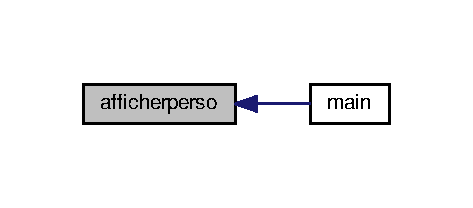
\includegraphics[width=227pt]{perso_8h_a47ed0411b9adbc7543d3e80815cb3401_icgraph}
\end{center}
\end{figure}


\index{perso.\+h@{perso.\+h}!animate\+Entity@{animate\+Entity}}
\index{animate\+Entity@{animate\+Entity}!perso.\+h@{perso.\+h}}
\subsubsection[{\texorpdfstring{animate\+Entity(personnage $\ast$pers)}{animateEntity(personnage *pers)}}]{\setlength{\rightskip}{0pt plus 5cm}void animate\+Entity (
\begin{DoxyParamCaption}
\item[{{\bf personnage} $\ast$}]{pers}
\end{DoxyParamCaption}
)}\hypertarget{perso_8h_ab3df315948613e2596ba989c3901ce00}{}\label{perso_8h_ab3df315948613e2596ba989c3901ce00}


to animate the personnage pers . 


\begin{DoxyParams}{Parameters}
{\em matrice} & \\
\hline
{\em pers} & the personnage \\
\hline
\end{DoxyParams}
\begin{DoxyReturn}{Returns}
Nothing 
\end{DoxyReturn}


Definition at line 93 of file perso.\+c.



References personnage\+::num.


\begin{DoxyCode}
94 \{
95 
96 \textcolor{keywordflow}{if}(pers->\hyperlink{structpersonnage_acfac32928075716cc10265cfc9f551fc}{num}==3)
97 pers->\hyperlink{structpersonnage_acfac32928075716cc10265cfc9f551fc}{num}=0;
98 \textcolor{keywordflow}{else} pers->\hyperlink{structpersonnage_acfac32928075716cc10265cfc9f551fc}{num}++;
99 
100 \}
\end{DoxyCode}


Here is the caller graph for this function\+:
\nopagebreak
\begin{figure}[H]
\begin{center}
\leavevmode
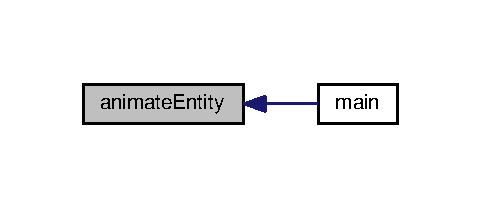
\includegraphics[width=231pt]{perso_8h_ab3df315948613e2596ba989c3901ce00_icgraph}
\end{center}
\end{figure}


\index{perso.\+h@{perso.\+h}!blit\+Entity@{blit\+Entity}}
\index{blit\+Entity@{blit\+Entity}!perso.\+h@{perso.\+h}}
\subsubsection[{\texorpdfstring{blit\+Entity(personnage $\ast$pers, S\+D\+L\+\_\+\+Surface $\ast$ecran)}{blitEntity(personnage *pers, SDL_Surface *ecran)}}]{\setlength{\rightskip}{0pt plus 5cm}void blit\+Entity (
\begin{DoxyParamCaption}
\item[{{\bf personnage} $\ast$}]{pers, }
\item[{S\+D\+L\+\_\+\+Surface $\ast$}]{ecran}
\end{DoxyParamCaption}
)}\hypertarget{perso_8h_ae3c5c8505cfb2638fa312c5cb8e20aa5}{}\label{perso_8h_ae3c5c8505cfb2638fa312c5cb8e20aa5}


to blit the surface of personnage pers . 


\begin{DoxyParams}{Parameters}
{\em pers} & the personnage \\
\hline
\end{DoxyParams}
\begin{DoxyReturn}{Returns}
Nothing 
\end{DoxyReturn}


Definition at line 157 of file perso.\+c.



References personnage\+::d, personnage\+::mat, personnage\+::num, and personnage\+::\+Positionmat.


\begin{DoxyCode}
158 \{
159 
160 SDL\_BlitSurface(pers->\hyperlink{structpersonnage_a7e7c398ea690ec57a5fce13c80386cd4}{mat}[pers->\hyperlink{structpersonnage_ad3316ca5e21971af05da3b10b0d18fb3}{d}][pers->\hyperlink{structpersonnage_acfac32928075716cc10265cfc9f551fc}{num}],NULL,ecran,&pers->
      \hyperlink{structpersonnage_a8216e2ba9fa8840fd13e47f40ccf356d}{Positionmat});
161 SDL\_Flip(ecran);
162 
163 \}
\end{DoxyCode}


Here is the caller graph for this function\+:
\nopagebreak
\begin{figure}[H]
\begin{center}
\leavevmode
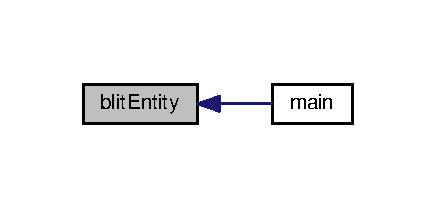
\includegraphics[width=209pt]{perso_8h_ae3c5c8505cfb2638fa312c5cb8e20aa5_icgraph}
\end{center}
\end{figure}


\index{perso.\+h@{perso.\+h}!deplacer\+\_\+perso@{deplacer\+\_\+perso}}
\index{deplacer\+\_\+perso@{deplacer\+\_\+perso}!perso.\+h@{perso.\+h}}
\subsubsection[{\texorpdfstring{deplacer\+\_\+perso(int direction, personnage $\ast$pers)}{deplacer_perso(int direction, personnage *pers)}}]{\setlength{\rightskip}{0pt plus 5cm}void deplacer\+\_\+perso (
\begin{DoxyParamCaption}
\item[{int}]{direction, }
\item[{{\bf personnage} $\ast$}]{pers}
\end{DoxyParamCaption}
)}\hypertarget{perso_8h_ac29231e5ad237f14aa979bd358003dec}{}\label{perso_8h_ac29231e5ad237f14aa979bd358003dec}


to move the personnage pers . 


\begin{DoxyParams}{Parameters}
{\em pers} & the personnage \\
\hline
\end{DoxyParams}
\begin{DoxyReturn}{Returns}
Nothing 
\end{DoxyReturn}


Definition at line 112 of file perso.\+c.



References personnage\+::\+Positionmat.


\begin{DoxyCode}
112                                                    \{
113     
114     \textcolor{keywordflow}{if}(direction==0)\{
115               
116               pers->\hyperlink{structpersonnage_a8216e2ba9fa8840fd13e47f40ccf356d}{Positionmat}.x+=25; 
117                    
118 \} 
119      \textcolor{keywordflow}{else} 
120          \textcolor{keywordflow}{if}(direction==1)\{ 
121                
122               pers->\hyperlink{structpersonnage_a8216e2ba9fa8840fd13e47f40ccf356d}{Positionmat}.x-=25; \}
123               
124 \textcolor{keywordflow}{else} \textcolor{keywordflow}{if}(direction==2)
125 \{
126 
127 pers->\hyperlink{structpersonnage_a8216e2ba9fa8840fd13e47f40ccf356d}{Positionmat}.x+=2;
128 
129 \}
130     
131 
132 
133 
134 \}
\end{DoxyCode}


Here is the caller graph for this function\+:
\nopagebreak
\begin{figure}[H]
\begin{center}
\leavevmode
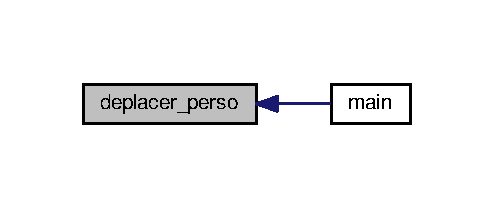
\includegraphics[width=237pt]{perso_8h_ac29231e5ad237f14aa979bd358003dec_icgraph}
\end{center}
\end{figure}


\index{perso.\+h@{perso.\+h}!init\+\_\+perso@{init\+\_\+perso}}
\index{init\+\_\+perso@{init\+\_\+perso}!perso.\+h@{perso.\+h}}
\subsubsection[{\texorpdfstring{init\+\_\+perso(personnage $\ast$pers)}{init_perso(personnage *pers)}}]{\setlength{\rightskip}{0pt plus 5cm}void init\+\_\+perso (
\begin{DoxyParamCaption}
\item[{{\bf personnage} $\ast$}]{pers}
\end{DoxyParamCaption}
)}\hypertarget{perso_8h_a21661aa89318d131d372cdacb5ef82c3}{}\label{perso_8h_a21661aa89318d131d372cdacb5ef82c3}


To initialize the \hyperlink{perso_8c}{perso.\+c}. 


\begin{DoxyParams}{Parameters}
{\em pers} & the personnage \\
\hline
{\em url} & the url of the image \\
\hline
\end{DoxyParams}
\begin{DoxyReturn}{Returns}
Nothing 
\end{DoxyReturn}


Definition at line 39 of file perso.\+c.



References personnage\+::acceleration, personnage\+::d, personnage\+::mat, personnage\+::nscore, personnage\+::num, personnage\+::nvie, personnage\+::\+Positionmat, personnage\+::up, and personnage\+::vitesse.


\begin{DoxyCode}
39                                  \{
40     pers->\hyperlink{structpersonnage_a7e7c398ea690ec57a5fce13c80386cd4}{mat}[0][0]=IMG\_Load(\textcolor{stringliteral}{"p.png"}); 
41         pers->\hyperlink{structpersonnage_a7e7c398ea690ec57a5fce13c80386cd4}{mat}[0][1]=IMG\_Load(\textcolor{stringliteral}{"p1.png"});
42         pers->\hyperlink{structpersonnage_a7e7c398ea690ec57a5fce13c80386cd4}{mat}[0][2]=IMG\_Load(\textcolor{stringliteral}{"p2.png"});
43         pers->\hyperlink{structpersonnage_a7e7c398ea690ec57a5fce13c80386cd4}{mat}[0][3]=IMG\_Load(\textcolor{stringliteral}{"p3.png"});  
44         pers->\hyperlink{structpersonnage_a7e7c398ea690ec57a5fce13c80386cd4}{mat}[1][0]=IMG\_Load(\textcolor{stringliteral}{"p4.png"});
45         pers->\hyperlink{structpersonnage_a7e7c398ea690ec57a5fce13c80386cd4}{mat}[1][1]=IMG\_Load(\textcolor{stringliteral}{"p5.png"});
46         pers->\hyperlink{structpersonnage_a7e7c398ea690ec57a5fce13c80386cd4}{mat}[1][2]=IMG\_Load(\textcolor{stringliteral}{"p6.png"});
47         pers->\hyperlink{structpersonnage_a7e7c398ea690ec57a5fce13c80386cd4}{mat}[1][3]=IMG\_Load(\textcolor{stringliteral}{"p7.png"});
48         pers->\hyperlink{structpersonnage_a7e7c398ea690ec57a5fce13c80386cd4}{mat}[2][0]=IMG\_Load(\textcolor{stringliteral}{"p10.png"});  
49         pers->\hyperlink{structpersonnage_a7e7c398ea690ec57a5fce13c80386cd4}{mat}[2][1]=IMG\_Load(\textcolor{stringliteral}{"p10.png"});
50         pers->\hyperlink{structpersonnage_a7e7c398ea690ec57a5fce13c80386cd4}{mat}[2][2]=IMG\_Load(\textcolor{stringliteral}{"p10.png"});
51         pers->\hyperlink{structpersonnage_a7e7c398ea690ec57a5fce13c80386cd4}{mat}[2][3]=IMG\_Load(\textcolor{stringliteral}{"p10.png"});
52 
53 pers->\hyperlink{structpersonnage_ad3316ca5e21971af05da3b10b0d18fb3}{d}=0;
54 pers->\hyperlink{structpersonnage_acfac32928075716cc10265cfc9f551fc}{num}=0;
55 pers->\hyperlink{structpersonnage_a8216e2ba9fa8840fd13e47f40ccf356d}{Positionmat}.x=0;
56 pers->\hyperlink{structpersonnage_a8216e2ba9fa8840fd13e47f40ccf356d}{Positionmat}.y=250;
57 pers->\hyperlink{structpersonnage_a5f78a81264a0d479a023826b20b86173}{nvie}=3; 
58 pers->\hyperlink{structpersonnage_a6c5c952d4dc96ed7f6be22480cb5a4d0}{nscore}=0; 
59 
60 pers->\hyperlink{structpersonnage_a9833848acdb28a307902c8e1682213d9}{vitesse}=5;
61 pers->\hyperlink{structpersonnage_aa3dc1bee3cdaa742eac0d46f56ac8908}{acceleration}=0;
62 pers->\hyperlink{structpersonnage_ad781b14c9d0a4f927e6471b9cf1234df}{up}=0;
63 
64 
65     
66 
67 
68 
69 
70 
71 
72 
73 
74 
75 \}
\end{DoxyCode}


Here is the caller graph for this function\+:
\nopagebreak
\begin{figure}[H]
\begin{center}
\leavevmode
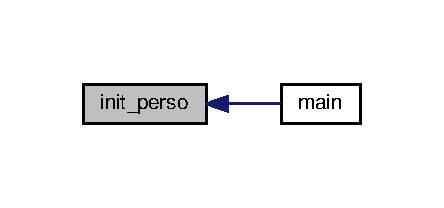
\includegraphics[width=213pt]{perso_8h_a21661aa89318d131d372cdacb5ef82c3_icgraph}
\end{center}
\end{figure}


\index{perso.\+h@{perso.\+h}!move\+Perso@{move\+Perso}}
\index{move\+Perso@{move\+Perso}!perso.\+h@{perso.\+h}}
\subsubsection[{\texorpdfstring{move\+Perso(personnage $\ast$pers, Uint32 dt)}{movePerso(personnage *pers, Uint32 dt)}}]{\setlength{\rightskip}{0pt plus 5cm}void move\+Perso (
\begin{DoxyParamCaption}
\item[{{\bf personnage} $\ast$}]{pers, }
\item[{Uint32}]{dt}
\end{DoxyParamCaption}
)}\hypertarget{perso_8h_aca4de1454b86bed715fb9f30706cd979}{}\label{perso_8h_aca4de1454b86bed715fb9f30706cd979}


to accelerate the personnage pers . 


\begin{DoxyParams}{Parameters}
{\em pers} & the personnage \\
\hline
\end{DoxyParams}
\begin{DoxyReturn}{Returns}
Nothing 
\end{DoxyReturn}


Definition at line 143 of file perso.\+c.



References personnage\+::acceleration, and personnage\+::vitesse.


\begin{DoxyCode}
144 \{
145 \textcolor{keywordtype}{double} dx;
146 dx=pers->\hyperlink{structpersonnage_a9833848acdb28a307902c8e1682213d9}{vitesse}*dt+0.5*pers->\hyperlink{structpersonnage_aa3dc1bee3cdaa742eac0d46f56ac8908}{acceleration}*dt*dt;
147 
148 \}
\end{DoxyCode}


Here is the caller graph for this function\+:
\nopagebreak
\begin{figure}[H]
\begin{center}
\leavevmode
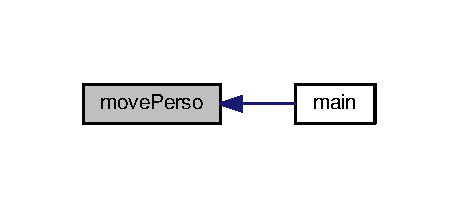
\includegraphics[width=220pt]{perso_8h_aca4de1454b86bed715fb9f30706cd979_icgraph}
\end{center}
\end{figure}


\index{perso.\+h@{perso.\+h}!saut@{saut}}
\index{saut@{saut}!perso.\+h@{perso.\+h}}
\subsubsection[{\texorpdfstring{saut(personnage $\ast$pers, int dt, int posint)}{saut(personnage *pers, int dt, int posint)}}]{\setlength{\rightskip}{0pt plus 5cm}void saut (
\begin{DoxyParamCaption}
\item[{{\bf personnage} $\ast$}]{pers, }
\item[{int}]{dt, }
\item[{int}]{posint}
\end{DoxyParamCaption}
)}\hypertarget{perso_8h_aa512e7feb8c56d184403ca02f0c094a7}{}\label{perso_8h_aa512e7feb8c56d184403ca02f0c094a7}


jump the personnage pers . 


\begin{DoxyParams}{Parameters}
{\em pers} & the personnage \\
\hline
\end{DoxyParams}
\begin{DoxyReturn}{Returns}
Nothing 
\end{DoxyReturn}


Definition at line 206 of file perso.\+c.



References personnage\+::acceleration, personnage\+::\+Positionmat, personnage\+::up, and personnage\+::vitesse.


\begin{DoxyCode}
207 \{
208 
209 \textcolor{keywordflow}{if}(pers->\hyperlink{structpersonnage_ad781b14c9d0a4f927e6471b9cf1234df}{up}==1)
210 \{
211 pers->\hyperlink{structpersonnage_a8216e2ba9fa8840fd13e47f40ccf356d}{Positionmat}.y-=80;
212 
213 
214 
215 \}
216 posint=pers->\hyperlink{structpersonnage_a8216e2ba9fa8840fd13e47f40ccf356d}{Positionmat}.y-=80;
217 
218 
219 \textcolor{keywordtype}{double} dx;
220 \textcolor{keywordflow}{if}(pers->\hyperlink{structpersonnage_a8216e2ba9fa8840fd13e47f40ccf356d}{Positionmat}.y==posint)
221 \{
222 
223 
224 pers->\hyperlink{structpersonnage_a8216e2ba9fa8840fd13e47f40ccf356d}{Positionmat}.y+=80;
225 
226 dx=0.5*pers->\hyperlink{structpersonnage_aa3dc1bee3cdaa742eac0d46f56ac8908}{acceleration} + 5*dt;
227 pers->\hyperlink{structpersonnage_a9833848acdb28a307902c8e1682213d9}{vitesse}-=dx;
228 \}
229 
230 
231 
232 
233 \}
\end{DoxyCode}


Here is the caller graph for this function\+:
\nopagebreak
\begin{figure}[H]
\begin{center}
\leavevmode
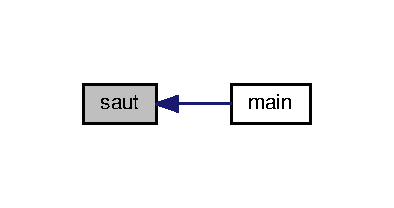
\includegraphics[width=189pt]{perso_8h_aa512e7feb8c56d184403ca02f0c094a7_icgraph}
\end{center}
\end{figure}




\subsection{Variable Documentation}
\index{perso.\+h@{perso.\+h}!pers@{pers}}
\index{pers@{pers}!perso.\+h@{perso.\+h}}
\subsubsection[{\texorpdfstring{pers}{pers}}]{\setlength{\rightskip}{0pt plus 5cm}{\bf personnage} pers}\hypertarget{perso_8h_a9665deb0dbbab88867dd0328603d3f32}{}\label{perso_8h_a9665deb0dbbab88867dd0328603d3f32}


Definition at line 27 of file perso.\+h.


%--- End generated contents ---

% Index
\backmatter
\newpage
\phantomsection
\clearemptydoublepage
\addcontentsline{toc}{chapter}{Index}
\printindex

\end{document}
